\documentclass{template/openetcs_article}
% Use the option "nocc" if the document is not licensed under Creative Commons
%\documentclass[nocc]{template/openetcs_article}
\usepackage{lipsum,url,color}
\usepackage{hyperref}
\graphicspath{{./template/}{.}{./images/}}
\begin{document}
\frontmatter
\project{openETCS}

%Please do not change anything above this line
%============================
% The document metadata is defined below

%assign a report number here
\reportnum{OETCS}

%define your workpackage here
\wp{Work-Package 7: ``Toolchain''}


\author{Uwe Steinke, Siemens AG}

\affiliation{Siemens AG}

\title{SCADE Model of Subset 026, Section 3.5, Management of Radio Communication (MoRC)}

% define the coverart
\coverart[width=350pt]{chart}

\reporttype{Model Description}


%\begin{document}

\maketitle
\tableofcontents
\listoffiguresandtables
\newpage

This document describes a formal model of the requirements of section~3.5 of
subset 026 of the ETCS specification 3.3.0. This section 
describes the management of a communication session between onboard and
on-track equipment from the view of the onboard unit (OBU).

The model is written in the (graphical) formal language SCADE by using the 
SCADE Suite, an integrated SCADE development environment. 

At the beginning of this document a short overview about the SCADE language and the SCADE development suite will be given. 

The following chapters introduce the "`Management of Radio Communication"' model to ease it's unterstanding. 

For a complete and detailed model description please refer to the MoRC document, generated from the model itself and located within this repository.

\newpage

\section{Short Introduction to Formalism and Tool}
\label{sec:short-intr-form}

\subsection{Motivation and Intention}
\label{sec:MotivationAndIntention}

The intention of SCADE is to provide a language and the appropriate development tool suite for embedded control software where high demands on dependability, reliability and safety are required. 

Therefore SCADE targets especially on safety related systems in the avionics, rail and automotive domain. 

SCADE provides certified code generators that transform the SCADE sources into executable C and ADA code. 


\subsection{SCADE Language and Formalism}
\label{sec:SCADELanguageAndFormalism}

SCADE is a formal textual and graphical language, where textual and graphical elements can be mixed with each other. The textual form is more applicable for automatized use, if the SCADE code itself should be generated from other tools. The graphical form is more intuitive and therefore suits better to manual modelling tasks. Within this document we will refer to the graphical representation. 

\subsubsection{The SCADE paradigm}
\label{sec:TheSCADEParadigm}

The SCADE language is based on one basic paradigm, that must be understood by it's users. 

\textbf{SCADE models are} 
\begin{quote}
\begin{itemize}

	\item synchronously
	\item clocked
	\item data flow and state machines and
	\item any nested combinations of these
	
\end{itemize}
\end{quote}


\begin{figure}[htbp]
	\centering
		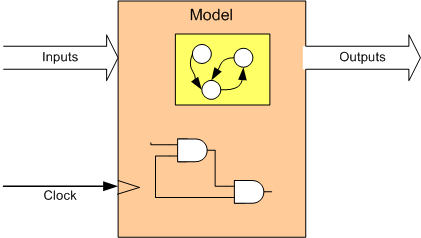
\includegraphics[width=0.65\textwidth]{SCADE_Paradigm.png}
	\caption{The SCADE Paradigm}
	\label{fig:SCADE_Paradigm}
\end{figure}

A clock cycle consist of these actions:
\begin{quote}
\begin{itemize}
	\item Apply input data to the model
	\item Compute / execute
	\item Disseminate model output data to external interfaces
\end{itemize}
\end{quote}

SCADE does not make any assumptions on the clock timing. A continuous aequidistant period clocking leads to implicite dependable timing relations, while discontinuous clocking often suits better to existing hardware platforms.  

In any case, the synchronous clocking principle causes a dependable timing behaviour of the model running on the target system without any racing and transient bug effects.


\subsubsection{SCADE Language}
\label{sec:SCADELanguage}

While SCADE models can be written as text, the more friendly way of modelling is the graphical schematic entry with the editor that comes as part of the SCADE Suite.

The intention of the SCADE language is not only to model the structure of a software application, where the software has to be implemented with other languages afterwards. Instead, SCADE models are the software implementation itself and in any case executable and verifyable. This is very different from modelling languages like SysML. On the other hand, the level of abstraction is below SysML.

The SCADE language provides all capabilities typically required for embedded control applications. It 
is based on strong data types like bool, integer, real, enumerations and structures and arrays of these. 

SCADE offers two fundamental concepts for modelling: (Data) flows and state machines.

\begin{figure}[htbp]
	\centering
		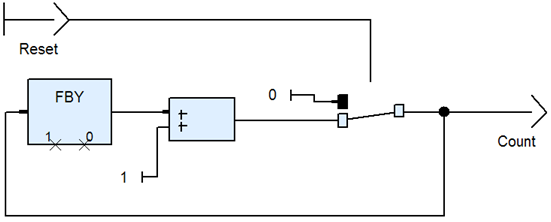
\includegraphics{DataFlow.png}
	\caption{SCADE data flow example}
	\label{fig:DataFlow}
\end{figure}

The data flow design are similar to electrical schematic diagrams and can be understood intuitively. 
Elementary operators for data flows are

\begin{quote}
	
\begin{itemize}
	\item boolean functions
	\item arithmetic functions
	\item choice (if/then/else, switch case, ...) 
  \item iterators over arrays of data, state machines and functions (map, fold)
  \item temporal operators (access to previous values of data flows)	
\end{itemize}
\end{quote}
 

\begin{figure}[htbp]
	\centering
		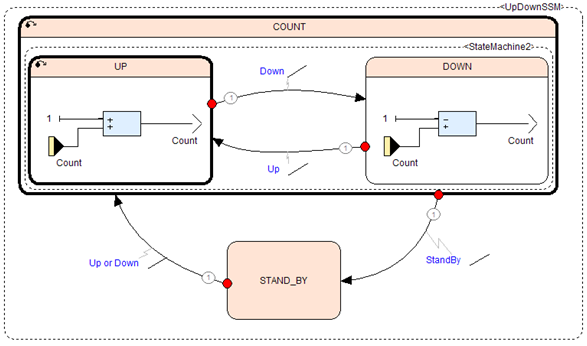
\includegraphics{StateMachine.png}
	\caption{Example of 2 nested state machines with data flows}
	\label{fig:StateMachine}
\end{figure}

State machines and data flows have completely deterministic semantics. For example, state transitions have unambiguous priorities for the case when more than one guard condition should be met. 

Data flows and state machines can be intermixed and parallelized and nested without limitations, which gives freedom to choose the more appropriate method for each model detail.

The SCADE language comprises some intentional restrictions that prevent the model designer from risky constructions in dependable and critical software applications: 

\begin{quote}
\begin{itemize}
	\item Static resource allocation only (no dynamic object creation at runtime)
	\item No recursions
	\item Loops / iterations with maximum repetition count only (no never ending loops)
\end{itemize}
\end{quote}
  

\newpage

\section{Modeling Strategy}
\label{sec:modeling-strategy}

The model implements the SRS Subset-026, section 3.5 "`Management of Radio Communication"'. 
This was achieved by modeling the subsections of the document one after the other subsequently in a clause-by-clause manner. 

The requirements text clauses were analyzed to identify the inputs and outputs of a subfunction und the task of the subfunction itself. The inputs and outputs were adopted as model in- and outputs directly and both interconnected by implementing the required task from inputs to outputs. 

This proceeding lead to a lot of small subfunctions. Then, the inputs and outputs of these subfunctions were matched so that outputs of subfunctions were connected to inputs of other subfunctions that required these kinds of information as inputs. 
At the end, the remaining inputs and outputs not connected within the model were taken as inputs and outputs of the whole model. 

\section{Model Overview}
\label{sec:model-overview}

The models top level operator is "`managementOfRadioCommunication"'. It incorporates a state machine "`CommunicationSession\_SM"' with its states reflecting the subsections of section 3.5 like "`Establishing a communication session"', "`Maintaining a communication session"' and "`Terminating a communication session"'.

\begin{figure}[htbp]
	\centering
		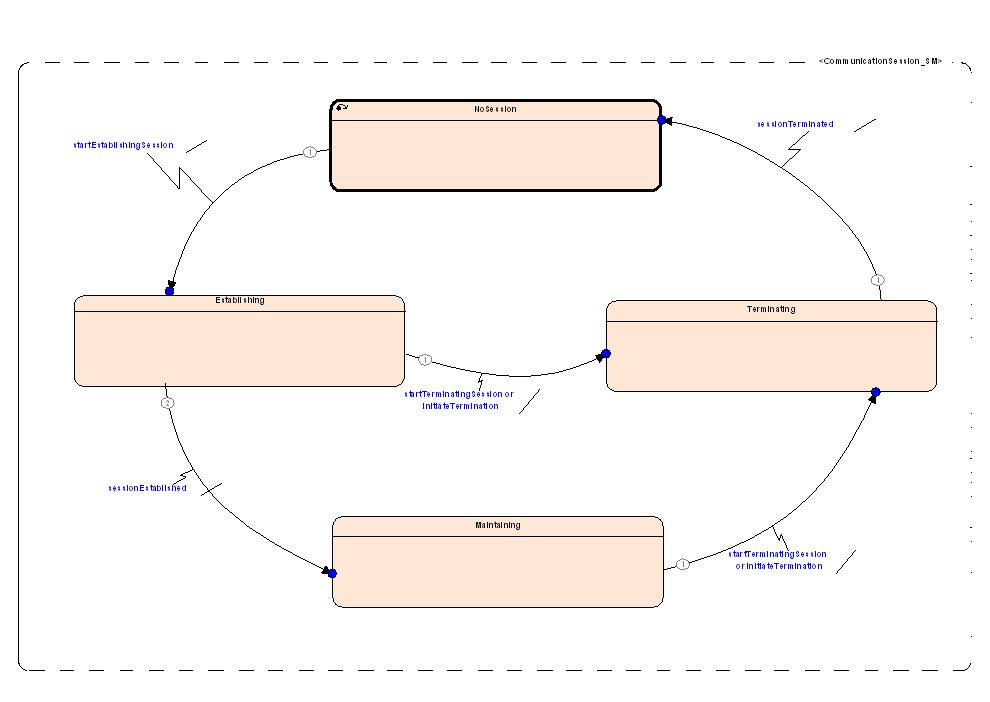
\includegraphics[width=0.65\textwidth]{CommunicationSessionSM.png}
	\caption{Session Management State Machine}
	\label{fig:CommunicationSessionSM}
\end{figure}

In parallel to the "`CommunicationSession\_SM"' state machine additional model nodes "`registeringToTheRadioNetwork"' and  "`safeRadioConnectionIndication"' directly correspond to further subsections of 3.5. The node "`initiateTerminatingASession"' assists in "`Terminating a communication session"'.


\begin{figure}[h]
	\centering
		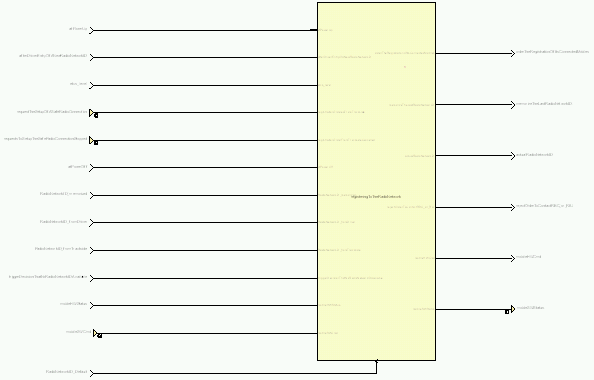
\includegraphics[width=0.65\textwidth]{networkRegistration.png}
	\caption{Registering to the Radio Network}
	\label{fig:networkRegistration}
\end{figure}

\begin{figure}[htbp]
	\centering
		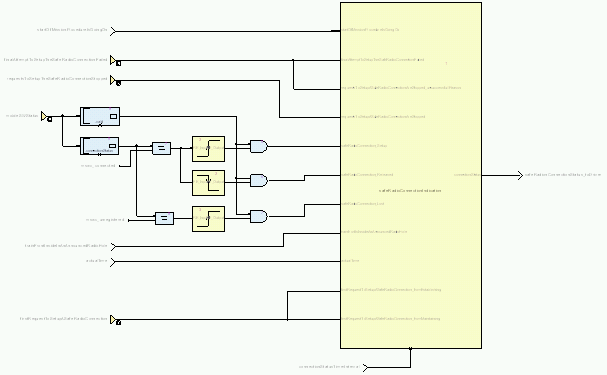
\includegraphics[width=0.65\textwidth]{safeRadioConnectionIndication.png}
	\caption{Indication of the Safe Radio  Connection}
	\label{fig:safeRadioConnectionIndication}
\end{figure}

\begin{figure}[htbp]
	\centering
		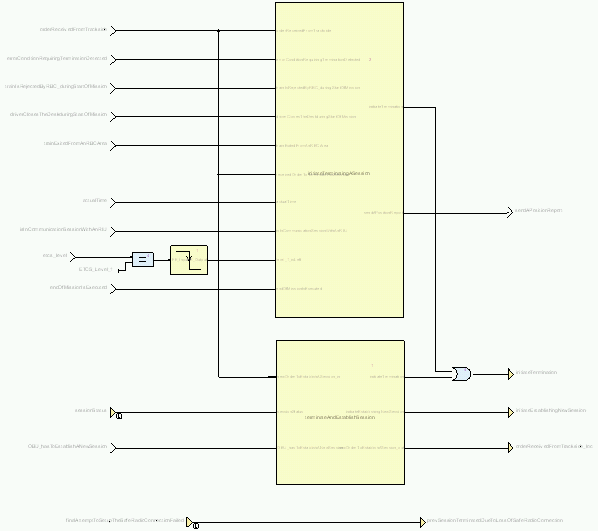
\includegraphics[width=0.65\textwidth]{InitiateTermination.png}
	\caption{Initiate terminating a Session}
	\label{fig:InitiateTermination}
\end{figure}

All 3.5 functions reside below the model top level layer as nested operators in "`managementOfRadioCommunication"'.
 
\clearpage

\section{Model Benefits}
\label{sec:model-highlights}

The described way of transformation from the written textual requirement specification in conjunction with the modelling technique leads to the following benefits:


\begin{quote}
	
	\begin{enumerate}
		\item The model is strictly formal and concrete. In opposite to semiformal modelling languages there is no room for unambiguousness or weaknesses.
		\item The model is the implementation. It is the implementation of the required functions (the textual requirement specification) as understood by the modelling persons.
		\item The model is executable, simulatable and verifiable. With the SCADE code generator, a runnable can be generated from the model. It is ready for debugging, simulation and test on (graphical) model level, so that the behavior of the modelled functions can be investigated practically. It can be executed on any platform for which a C- or ADA compiler exists. This applies to the whole model as well to its subfunctions, which eases incremental and iterative development processes.
		\item To achieve requirements traceability, the model artefacts can be linked with the requirements located in the textual specification in fine granularity
		\item By applying description and explanations within the model, a documentation can be generated from it automatically.
		\item For integration into different toolchains, the tools are usable via command line and automatization interfaces, providing model information and meta-information, and there are plugins for eclipse.
		\item The tools, especially the code generator,  are qualified for safety-related software development compliant to DO-178B/Level a and CENELEC EN50128/SIL4.
		\item The language and tool chain are mature, efficient and complete.
	\end{enumerate}
	
\end{quote}

Some drawbacks of the shown proceeding:

\begin{quote}
	
	\begin{enumerate}
		\item Since the model originates from written requirements document, its structure is close to the documents structure. This cannot be expected to be optimal from the system or architectural point of view.
		\item The modeling language and technique is very suitable for the chosen target. For more complex systems like the whole ETCS OBU, a more abstract, less formal model and language intermediate layer like SysML might be appropriate between the textual specification and the SCADE model layer.
	\end{enumerate}
	
\end{quote}


\section{Detailed Model Description}
\label{sec:deta-model-descr}

A detailed descripted was generated from the model itself: \href{https://github.com/openETCS/model-evaluation/blob/master/model/SCADE_Siemens/Subset_026_Chapt_3.5_ManagementOfRadioCommunication/Generated_Documents/MoRC.pdf}{Management\_of\_Radio\_Communication}

\end{document}


%%% Local Variables:
%%% mode: latex
%%% TeX-master: t
%%% End:
